\section{Challenge 3 Level 2 (C3L2): RISCV-DV Test Coverage Enhancement}

\subsection{Introduction}
The objective of this activity was to improve test coverage in the RISCV-DV tool for the rv32i ISA. Despite various configurations being tested and evaluated, achieving 100\% coverage was challenging due to time constraints, lack of documentation, and limited knowledge of the tool.

\subsection{Test Generation and Interaction}
RISCV-DV was used for test generation with the following command:

\begin{verbatim}
run --target rv32i --test riscv_arithm
etic_basic_test --testlist testlist.yaml
--simulator pyflow
\end{verbatim}

To control the number of tests, the \texttt{-i} (interaction) parameter was utilized. For instance:

\begin{verbatim}
run --target rv32i --test riscv_arithm
etic_basic_test --testlist testlist.yaml
--simulator pyflow -v -i 50
\end{verbatim}

This command generated 50 tests as observed in Figure \ref{fig:run1}.

\begin{figure}[h]
  \centering
  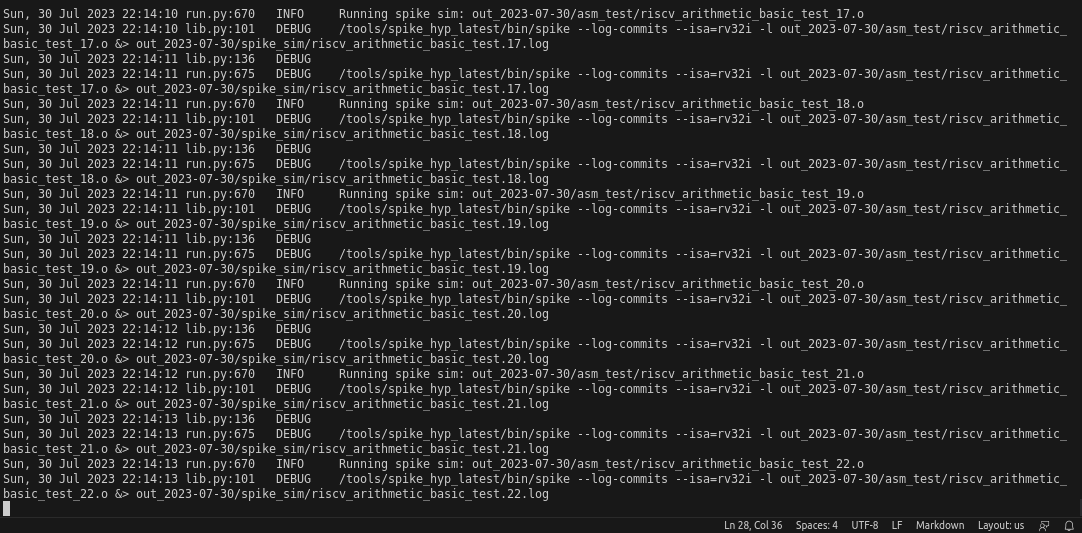
\includegraphics[width=0.5\textwidth]{./c3l2_img/run1.png}
  \caption{Test Generation with Interaction}
  \label{fig:run1}
\end{figure}

\subsection{Test Analysis and Coverage}
The generated tests can be analyzed as shown in Figure \ref{fig:run2}.

Coverage information can be obtained using the \texttt{cov} tool with the command below. The resulting output is depicted in Figure \ref{fig:run3}.

\begin{verbatim}
cov --dir out_*/spike_sim --enable_visua
lization  --simulator pyflow
\end{verbatim}

To analyze the coverage metrics, it is necessary to read the \texttt{CoverageReport.txt} in the \texttt{cov\_*/} folder, as demonstrated in Figure \ref{fig:run4}.

\subsection{Conclusion and Next Steps}
While various configurations were tested and evaluated, achieving 100\% coverage was not realized due to the limited availability of documentation, time constraints, and unfamiliarity with the tool.

For future improvements, it is essential to explore the tool's documentation and seek assistance from the community to address the coverage issues efficiently. Additionally, further analysis of uncovered areas in the ISA and targeted test generation could be performed to enhance coverage results.

\begin{figure}[h]
  \centering
  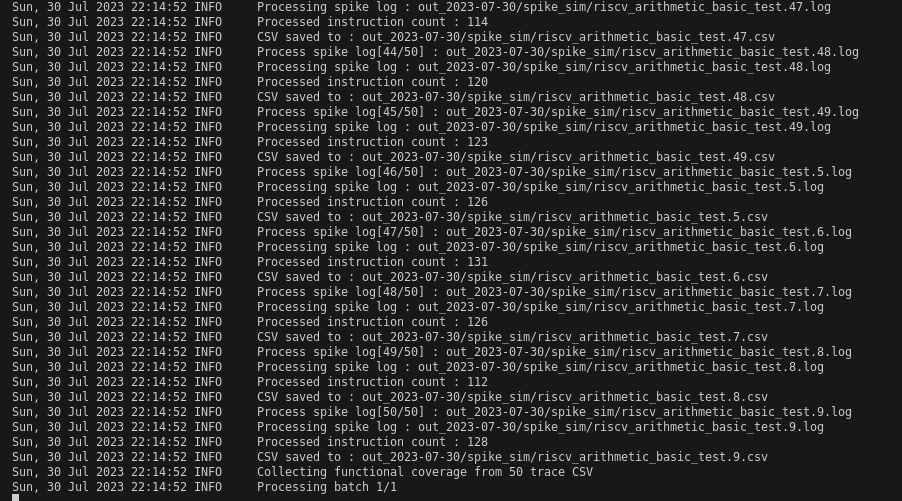
\includegraphics[width=0.5\textwidth]{./c3l2_img/run3.png}
  \caption{Coverage Report}
  \label{fig:run3}
\end{figure}

\begin{figure}[h]
  \centering
  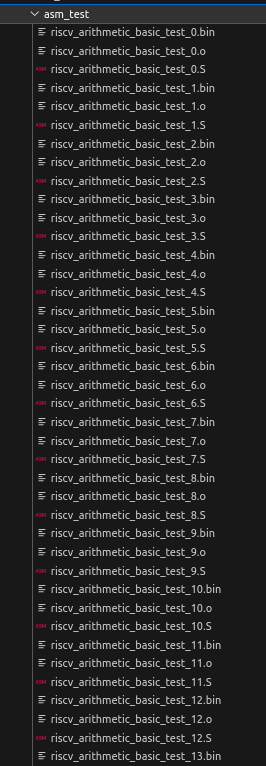
\includegraphics[width=0.21\textwidth]{./c3l2_img/run2.png}
  \caption{Test Analysis}
  \label{fig:run2}
\end{figure}


\begin{figure}[h]
  \centering
  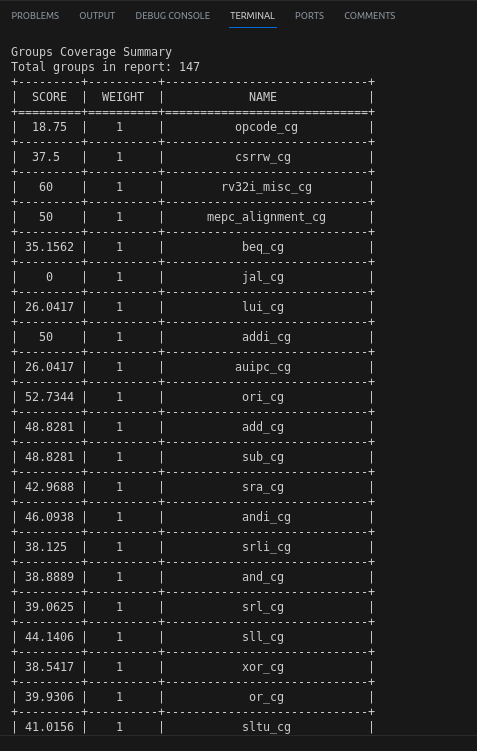
\includegraphics[width=0.19\textwidth]{./c3l2_img/run4.png}
  \caption{Coverage Metrics}
  \label{fig:run4}
\end{figure}

